\section{Theorie}

\section{Zielsetzung}
    Das Ziel dieses Versuchs ist es die Aufspaltung der Zeeman-Niveaus und ihre Polarisation zu untersuchen.
    Dabei werden die Aufspaltung einer $\ce{Cd}$-Spektrallampe unter Einfluss eines Magnetfeldes untersucht.
\section{Theorie}

\subsection{Energielevelstruktur}


\subsubsection{Die einfachen Niveaus und die Feinstruktur}

\noindent
Die Energieniveaus der Valenzelektronen hängt in erster Ordnung von der Hauptquantenzahl $n$ ab, 
welche beschreibt im wievielten angeregten Zustand sich ein Elektron befindet.\\
Für jeden dieser Zustände kann das Elektron unterschiedliche Bahndrehimpulse annehmen. Genauer gilt $l \in \{0,1, ..., n-1\}$. Im energetischen Grundzustand gilt also $l = 0$.\\
Dieser Effekt hat die größten Energiedifferenzen $\increment E$ zwischen seinen Niveaus.
Der Betrag des Bahndrehimpulsvektors ist
\begin{equation*}
    |\vec{l}| = \hbar \sqrt{l(l+1)} \quad .
\end{equation*}\\\\
Dies sind aber nicht alle Effekte, die zur Aufspaltung der Energieniveaus der Elektronen beitragen.
Des Weiteren muss noch beachtet werden, dass der Elektronenspin $s =\frac{1}{2}$ an seinen Bahndrehimpuls koppelt.
Dabei hat der Spinvektor den Betrag 
\begin{equation*}
    |\vec{s}| = \hbar \sqrt{s(s+1)} \quad .
\end{equation*}
Dies ist die sogenannte Spin-Bahn-Kopplung, welche Teil der Feinstruktur ist. \\
Stark vereinfacht gesagt wechselwirkt der Elektronenspin mit dem Magnetfeld, dass durch seine Bewegung entsteht, wodurch sich die Energieniveaus in $s$ und $l$ aufspalten.\\
Die Aufspaltung kann dabei durch $J$, den Spin der gesamten Schale beschrieben werden. Dabei kann $J$ Werte von $\bigl| L - S \bigr|$ bis $\bigl| L + S \bigr|$ annehmen.\\
Im Vergleich mit den $n$-Niveaus sind die Energiedifferenzen deutlich kleiner.\\\\

\noindent
Dieser Effekt tritt so aber nur für Atome mit einem Valenzelektron oder einer hohen Ordnungszahl auf. Für die großen Atome wird er \textbf{jj-Kopplung} genannt. 
Wenn sich bei einem solchen Atom mehrere Elektronen auf der äußersten Schale befinden, werden die einzelnen Elektronen über den Kern stark voneinander abgeschirmt.
Die Wechselwirkung der Spins mit dem eigenen Bahndrehimpuls ist also größer als die der Elektronen untereinander.
Aus diesem Grund wird für die Bestimmung des Gesamtdrehimpulses der Schale $J$ über die Gesamtdrehimpulse der einzelnen Elektronen $\vec j_\t{i} = \vec{l}_\t{i} + \vec{s}_\t{i}$ 
summiert mit 
\begin{equation*}
    \vec J = \sum_i \vec j_\t{i} \quad.
\end{equation*}
Für Atome mit geringerer Ordnungszahl ist das Gegenteil der Fall. Hier dominiert die Wechselwirkung der Elektronen untereinander. 
Dies wird die \textbf{LS-Kopplung} genannt. Der Gesamtdrehimpuls $\vec J $ ergibt sich über 
\begin{align}
    \vec{J} &= \vec{L} + \vec{S} & |\vec{J}| = \hbar \sqrt{J(J+1)}\\
    \intertext{mit}
    \vec{L} &= \sum_i \vec{l_i}  & |\vec{L}| = \hbar \sqrt{L(L+1)}\\
    \vec{S} &= \sum_i \vec{s_i}  & |\vec{S}| = \hbar \sqrt{S(S+1)}.
\end{align}\\

\noindent
Den Drehimpulsen lassen sich magnetische Momente zuordnen. Für die Quantenzahlen $s$ und $l$ ergibt sich dabei 
\begin{align*}
    \vec{\mu_\t{l}} &= - \frac{\mu_\text{B}}{\hbar} \cdot \vec{l}, & |\vec{\mu_\t{l}}|& = - \mu_\text{B} \sqrt{l(l+1)}\\
    \vec{\mu_\t{s}} &= - g_\t{s} \frac{\mu_\text{B}}{\hbar} \cdot \vec{s}, & |\vec{\mu_\t{s}}| &= - g_\t{s} \mu_\text{B} \sqrt{s(s+1)} \quad ,
\end{align*}
wobei $\mu_\t{B}$ das Bohrsche Magneton ist.
Dies setzt sich aus 
\begin{equation*}
    \mu_\t{B} = \frac{\symup e \symup \hbar}{2\symup{m_e}}
\end{equation*}
zusammen. $\symup e$  ist die Elektronenladung\cite{e0}, $\symup \hbar$ das reduzierte Plancksche Wirkungsquantum\cite{Planck} und $\symup{m_e}$ die Elektronenmasse\cite{m0}.\\
In der LS-Kopplung lässt sich daraus das Gesamtmoment für die Schale über
%\begin{align*}
%    |\vec{\mu_L}|& = \mu_\text{B} \sqrt{L(L+1)} \:, &  |\vec{\mu_S}|& = g_\t{S} \mu_\text{B} \sqrt{S(S+1)}
%\end{align*}
\begin{align}
    \vec{\mu_J} &= \vec{\mu_L} + \vec{\mu_S} & |\vec{\mu_J}| = g_\t{J} \mu_\text{B} \sqrt{J(J+1)} 
\end{align}
berechnen. Dabei ist $g_\t{J} $ das gyromagnetische Verhältnis oder der Landé-Faktor 
\begin{equation}
    g_\t{J} = \frac{3J(J+1) + S(S+1) - L(L+1)}{2J(J+1)} \quad .
    \label{eqn:lande}
\end{equation}
Außerdem ist zu beachten, dass der Gesamtdrehimpuls $ \vec J$ oft nicht parallel zu $\mu_\t{J}$ steht.

\subsubsection{Der normale Zeeman-Effekt}

\noindent
Wenn nun ein externes Magnetfeld angelegt wird, tritt noch eine weitere Aufspaltung auf.
Dies ist der sogenannte Zeeman-Effekt und er hebt die Entartung der Energie in der magnetischen Quantenzahl $m$ auf.\\
Diese Quantenzahl beschreibt dabei die Projektion des Spins auf das externe Magnetfeld. 
Je nach Orientierung von $\vec J$ ist die Stärke der Kopplung zwischen magnetischem Moment und Magnetfeld also unterschiedlich.
$m$ hat dabei die $2J+1$ Eigenwerte von $-J$ bis $J$.\\
Für kleine externe Magnetfelder $B$  ergeben sich die Zeeman-Niveaus zu 
\begin{equation}
    E_\t{Z} = g_\t{J}\; \mu_B \; m \;\bigl| B \bigr|\quad .
    \label{eqn:zeeman}
\end{equation}
Sie beschreiben dabei die Abweichung von den Feinstruktur-Niveaus in Abhängigkeit von der Stärke des Magnetfelds $\bigl| B \bigr|$, 
der magnetischen Quantenzahl $m$, dem Bohrschen Magneton $\mu_\t{B}$ und dem gyromagnetischen Verhältnis oder auch Landé-Faktor $g_J$.\\
Für den normalen Zeeman-Effekt besitzen die Elektronen auf der äußeren Schale einen Gesamtspin $S=0$, womit $g_\t{J} = 1$ gilt.
Die Energieniveaus für den normalen Zeeman-Effekt sind in \autoref{img:normzee} schematisch aufgetragen.
\begin{figure}[H]
    \centering
    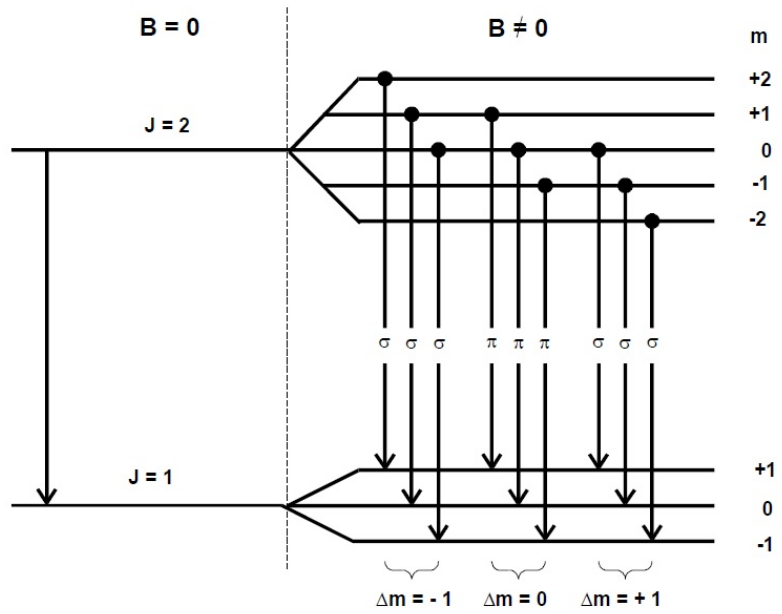
\includegraphics[width=0.6\textwidth]{latex/images/normalerzeeman.PNG}
    \caption{Die Energieniveaus des normalen Zeeman-Effekts inklusive der möglichen optischen Übergänge schematisch dargestellt \protect \cite{alt}.}
    \label{img:normzee}
\end{figure}

\subsubsection{Auswahlregeln der optischen Übergänge}

\noindent 
Wie in \autoref{img:normzee} und \autoref{img:annormzee} dargestellt, existieren zwischen den Zeemanniveaus eines angeregten und eines nicht angeregten Zustandes optische Übergänge.
Dabei ist allerdings zu beachten das nicht alle Übergänge erlaubt sind. 
Die Elektronen können über die spontane Emission eines Photons aus dem angeregten in den Grundzustand zerfallen.
Da das externe Magnetfeld allerdings die Entartung in $m$ aufhebt, sind bei Zerfällen aus den Niveaus der angeregten Zustände nur die möglich, bei denen $\increment m = \pm 1, 0$ gilt.
Dies lässt sich damit Begründen, dass ein Photon als Boson einen Gesamtdrehimpuls von $\pm 1, 0 $ annehmen kann, wodurch dies die einzigen Übergänge sind, die Drehimpulserhaltung nicht verletzen.\\
Übergänge mit $\increment m = 0$ senden dabei $\pi$-polarisiertes Licht aus, was linear-polarisiert bedeutet. 
Das für $\increment m = \pm 1$ ausgesendete zirkular-polarisierte Licht, wird mit $\sigma^{\pm}$ benannt.\\
Wie in Abbildung \autoref{img:pol} dargestellt unterscheiden sich die Aufspaltungsbilder der Spektrallinien abhängig davon, ob ein Magnetfeld anliegt und von dem Beobachtungswinkel.
Für ein deaktiviertes Magnetfeld existiert nur der Übergang zwischen den Niveaus von $J$, weswegen dort nur $\pi$-polarisiertes Licht emittiert wird, was der Linie in der Mitte entspricht.
Bei Betrachtung entlang des Magnetfeldes, in longitudinaler Richtung, ist das $\pi$-polarisierte Licht nicht zu erkennen, da sein Wellenvektor senkrecht zum Feld schwingt.
Für die transversale Richtung, orthogonal zum Feld, sind alle Linien zu erkennen. Da die zirkulare Polarisation allerdings auf diese Ebene projiziert wird erscheint es linear.


\begin{figure}[H]
    \centering
    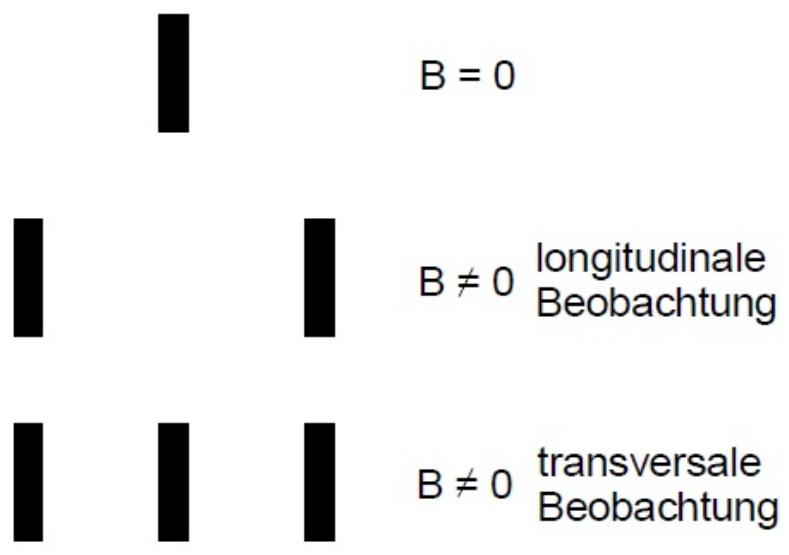
\includegraphics[width=0.4\textwidth]{latex/images/polarisation.PNG}
    \caption{Die Aufspaltungsbilder der optischen Übergänge in Abhängigkeit vom Beobachtungswinkel \protect \cite{alt}.}
    \label{img:pol}
\end{figure}


\subsubsection{Der anomale Zeeman-Effekt}

\noindent
Für den anomalen Zeeman-Effekt werden die Zustände berücksichtigt, für die $S \neq 0$ gilt. 
Damit gilt auch $g_\t{J} \neq 1$, wobei dieser nun wieder abhängig von $S$, $L$ und $J$ ist. 
Damit ergibt sich für die anomalen Zeemanniveaus 
\begin{equation}
    E_\t{aZ} = \underbrace{(m_1 g(L_1,\, S_1,\, J_1) - m_2 g(L_2,\, S_2,\, J_2))}_{= g_{1,2}} \mu_\text{B} |\vec{B}| \quad .
    \label{eqn:anorm}
\end{equation}
Dabei geben die Indices die Zugehörigkeit zu den unterschiedlichen Niveaus an.\\
In \autoref{img:annormzee} sind diese Übergänge schematisch dargestellt. 
Dabei gelten immer noch die Auswahlregeln für die optischen Übergänge. 
\begin{figure}[H]
    \centering
    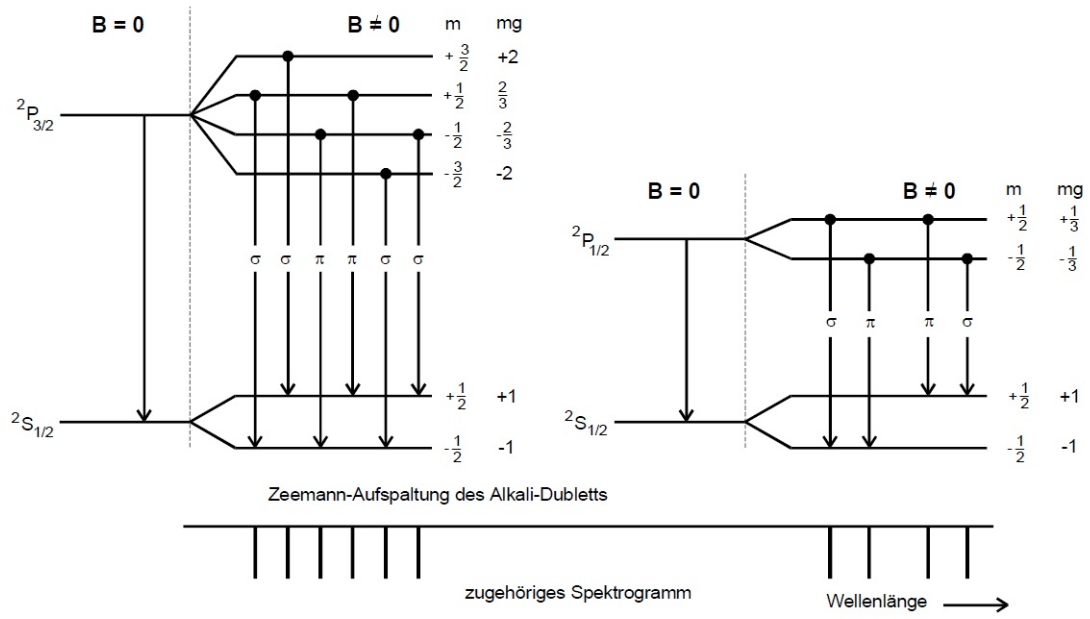
\includegraphics[width=0.8\textwidth]{latex/images/anormalerzeeman.PNG}
    \caption{Die Energieniveaus des anomalen Zeeman-Effekts inklusive der optischen Übergänge schematisch dargestellt.
    Außerdem sind noch die Aufspaltungsbilder der Übergänge aufgetragen \protect \cite{alt}.}
    \label{img:annormzee}
\end{figure}